\documentclass[t]{beamer}

\setlength {\marginparwidth }{2cm} 
\usepackage{todonotes}
\usepackage{siunitx}
\usepackage{subcaption}
\usepackage{apacite} 	% Use APA Citation
\presetkeys{todonotes}{inline}{}
\beamertemplatenavigationsymbolsempty

\usepackage{enumitem}

% \usetheme{AnnArbor}
% \usetheme{Antibes}
% \usetheme{Bergen}
% \usetheme{Berkeley}https://www.sharelatex.com/project/5b12e1a4f84b363f6f336dab
% \usetheme{Berlin}
% \usetheme{Boadilla}
% \usetheme{boxes}
\usetheme{CambridgeUS}
% \usetheme{Copenhagen}
%\usetheme{Darmstadt}
% \usetheme{default}
%\usetheme{Frankfurt}
%\usetheme{Goettingen}
% \usetheme{Hannover}
% \usetheme{Ilmenau}
% \usetheme{JuanLesPins}
\setlength{\parskip}{10pt}

% \newcommand*\vc[1]%
% {\begin{pmatrix}#1\end{pmatrix}}

\newcommand*\vc[1]%
{\left(\begin{array}{cccc}#1\end{array}\right)}


\newcommand\eqdef{\ \mathrel{\overset{\makebox[0pt]{\mbox{\normalfont\scriptsize\sffamily def}}}{=}}\ }

\title[Eligibility propagation]{Improving eligibility propagation using Izhikevich neurons in a multilayer RSNN.\\\vspace{10pt}
\large{Presentation 1: Formalizing the framework \& initial steps}}

\author[Werner]{Werner~van~der~Veen\\\tiny\texttt({w.k.van.der.veen.2@umcg.nl})}\date{\today}

\subject{Morphological Processing}

% \pgfdeclareimage[height=1cm]{umcg-logo}{umcg.png}
% \newif\ifplacelogo
% \placelogotrue
% \logo{\ifplacelogo\pgfuseimage{umcg-logo}\fi}

\begin{document}

\begin{frame}
    \titlepage
\end{frame}

%======================================

% \begin{frame}
%     \tableofcontents
% \end{frame}

\small
\section{Introduction: prior research summarized}

\begin{frame}{Bellec's e-prop}
    Bellec, G., Scherr, F., Subramoney, A., Hajek, E., Salaj, D., Legenstein, R., \& Maass, W. (2020). A solution to the learning dilemma for recurrent networks of spiking neurons.
    
    E-prop derived from BPTT:
    \begin{align}
        \frac{dE}{dW_{ji}} 
        &\eqdef \sum_t\frac{dE}{dz_j^t} & &\cdot\left[\frac{dz^t_j}{dW_{ji}}\right]_\text{local}&\\
        &\eqdef \sum_tL_j^t & &\cdot e^t_{ji}&\\
        &\eqdef \sum_t\sum_kB_{jk}\left(y_k^t-y_k^{*,t}\right) & &\cdot \frac{\partial z^t_j}{\partial \mathbf{h}^t_j}\left(\frac{\partial \mathbf{h}_j^t}{\partial\mathbf{h}_j^{t-1}}\cdot\mathbf{\epsilon}_{ji}^{t-1} + \frac{\partial\mathbf{h}^t_j}{\partial W_{ji}}\right)&
    \end{align}
\end{frame}

\begin{frame}{Bellec Architecture}
    \begin{figure}
    \centering
    \begin{subfigure}{.6\textwidth}
      \centering
      \includegraphics[width=\textwidth]{imgs/net.png}
    \end{subfigure}%
    \begin{subfigure}{.4\textwidth}
      \centering
      \includegraphics[width=.9\textwidth]{imgs/net2.png}
      \label{fig:sub2}
    \end{subfigure}
    \end{figure}
    
\end{frame}

\begin{frame}{Traub}
    Traub, M, Butz, M. V., Baayen, R. H., \& Otte, S. (2020). Learning Precise Spike Timings with Eligibility Traces.

    Corrects STDP behavior for negative learning.
    
    For (A)LIF, this is realized when hard resetting $v$ to zero after refractory period, because this automatically resets $e$.
    
    Izhikevich neurons naturally incorporate refractory periods and don't necessitate explicit refractory resets.
    \begin{align*}
        \tilde{u}^t_j &= v^t_j - \left(v^t_j + 65)z^t_j\right)\\
        \tilde{v}^t_j &= u^t_j + 2z^t_j\\
        u^{t+1}_j &= \tilde{u}^t_j + \delta t\left(0.004\tilde{v}^t_j - 0.02\tilde{u}^t_j\right)\\
        v^{t+1}_j &= \tilde{v}_j^t + \delta t\left(0.04\left(\tilde{v}^t_j\right)^2+5\tilde{v}^t_j + 140 - \tilde{u}^t_j + I^t_j\right)
    \end{align*}
    
\end{frame}
\begin{frame}{Izhikevich e-prop simulation}
    
    \begin{figure}
        \centering
        \includegraphics[width=.8\textwidth]{imgs/traub.png}
    \end{figure}
\end{frame}

\section{My idea}

\begin{frame}{My own idea: multilayer Izhikevich}
    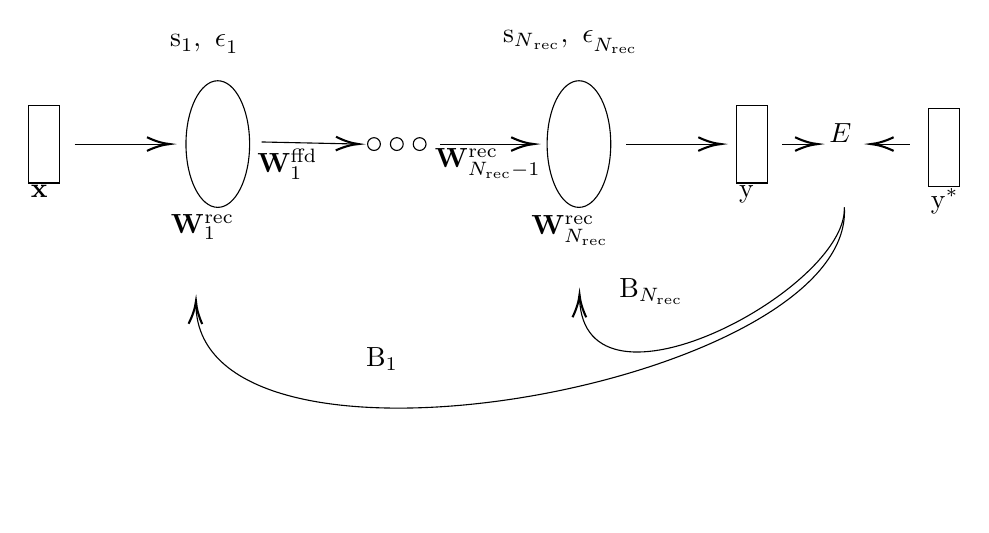
\begin{tikzpicture}[x=0.75pt,y=0.75pt,yscale=-1,xscale=1]
%uncomment if require: \path (0,276); %set diagram left start at 0, and has height of 276

%Shape: Rectangle [id:dp1936715011368968] 
\draw   (120.5,115.24) -- (135.46,115.24) -- (135.46,152.77) -- (120.5,152.77) -- cycle ;
%Straight Lines [id:da29874320875011495] 
\draw    (142.91,134.01) -- (186.66,134.01) ;
\draw [shift={(188.66,134.01)}, rotate = 180] [color={rgb, 255:red, 0; green, 0; blue, 0 }  ][line width=0.75]    (10.93,-3.29) .. controls (6.95,-1.4) and (3.31,-0.3) .. (0,0) .. controls (3.31,0.3) and (6.95,1.4) .. (10.93,3.29)   ;
%Shape: Ellipse [id:dp3402697204463556] 
\draw   (196.5,134.01) .. controls (196.5,117.16) and (203.36,103.5) .. (211.83,103.5) .. controls (220.3,103.5) and (227.16,117.16) .. (227.16,134.01) .. controls (227.16,150.85) and (220.3,164.51) .. (211.83,164.51) .. controls (203.36,164.51) and (196.5,150.85) .. (196.5,134.01) -- cycle ;
%Straight Lines [id:da8494502316670833] 
\draw    (233,133) -- (277.66,133.96) ;
\draw [shift={(279.66,134.01)}, rotate = 181.24] [color={rgb, 255:red, 0; green, 0; blue, 0 }  ][line width=0.75]    (10.93,-3.29) .. controls (6.95,-1.4) and (3.31,-0.3) .. (0,0) .. controls (3.31,0.3) and (6.95,1.4) .. (10.93,3.29)   ;
%Shape: Circle [id:dp22072610353797772] 
\draw   (284,134.01) .. controls (284,132.31) and (285.38,130.93) .. (287.08,130.93) .. controls (288.78,130.93) and (290.16,132.31) .. (290.16,134.01) .. controls (290.16,135.71) and (288.78,137.09) .. (287.08,137.09) .. controls (285.38,137.09) and (284,135.71) .. (284,134.01) -- cycle ;
%Shape: Circle [id:dp30793589859589243] 
\draw   (295,134.01) .. controls (295,132.31) and (296.38,130.93) .. (298.08,130.93) .. controls (299.78,130.93) and (301.16,132.31) .. (301.16,134.01) .. controls (301.16,135.71) and (299.78,137.09) .. (298.08,137.09) .. controls (296.38,137.09) and (295,135.71) .. (295,134.01) -- cycle ;
%Shape: Circle [id:dp8663350540407548] 
\draw   (306,134.01) .. controls (306,132.31) and (307.38,130.93) .. (309.08,130.93) .. controls (310.78,130.93) and (312.16,132.31) .. (312.16,134.01) .. controls (312.16,135.71) and (310.78,137.09) .. (309.08,137.09) .. controls (307.38,137.09) and (306,135.71) .. (306,134.01) -- cycle ;
%Straight Lines [id:da879536294691629] 
\draw    (318.91,134.01) -- (362.11,134.01) ;
\draw [shift={(364.11,134.01)}, rotate = 180] [color={rgb, 255:red, 0; green, 0; blue, 0 }  ][line width=0.75]    (10.93,-3.29) .. controls (6.95,-1.4) and (3.31,-0.3) .. (0,0) .. controls (3.31,0.3) and (6.95,1.4) .. (10.93,3.29)   ;
%Shape: Ellipse [id:dp5786629669544072] 
\draw   (370.5,134.01) .. controls (370.5,117.16) and (377.36,103.5) .. (385.83,103.5) .. controls (394.3,103.5) and (401.16,117.16) .. (401.16,134.01) .. controls (401.16,150.85) and (394.3,164.51) .. (385.83,164.51) .. controls (377.36,164.51) and (370.5,150.85) .. (370.5,134.01) -- cycle ;
%Straight Lines [id:da3180396189686683] 
\draw    (408.51,134.01) -- (452.26,134.01) ;
\draw [shift={(454.26,134.01)}, rotate = 180] [color={rgb, 255:red, 0; green, 0; blue, 0 }  ][line width=0.75]    (10.93,-3.29) .. controls (6.95,-1.4) and (3.31,-0.3) .. (0,0) .. controls (3.31,0.3) and (6.95,1.4) .. (10.93,3.29)   ;
%Shape: Rectangle [id:dp07787703444114347] 
\draw   (461.7,115.24) -- (476.66,115.24) -- (476.66,152.77) -- (461.7,152.77) -- cycle ;
%Straight Lines [id:da27112351293968695] 
\draw    (483.71,134.01) -- (498.91,134.01) ;
\draw [shift={(500.91,134.01)}, rotate = 180] [color={rgb, 255:red, 0; green, 0; blue, 0 }  ][line width=0.75]    (10.93,-3.29) .. controls (6.95,-1.4) and (3.31,-0.3) .. (0,0) .. controls (3.31,0.3) and (6.95,1.4) .. (10.93,3.29)   ;
%Straight Lines [id:da21989248518407156] 
\draw    (545.31,134.01) -- (528.51,134.01) ;
\draw [shift={(526.51,134.01)}, rotate = 360] [color={rgb, 255:red, 0; green, 0; blue, 0 }  ][line width=0.75]    (10.93,-3.29) .. controls (6.95,-1.4) and (3.31,-0.3) .. (0,0) .. controls (3.31,0.3) and (6.95,1.4) .. (10.93,3.29)   ;
%Shape: Rectangle [id:dp9261444093144608] 
\draw   (554.1,116.84) -- (569.06,116.84) -- (569.06,154.37) -- (554.1,154.37) -- cycle ;
%Curve Lines [id:da017874895307963712] 
\draw    (513.71,164.51) .. controls (515.29,203.71) and (388.29,271.54) .. (386.14,208.46) ;
\draw [shift={(386.11,206.51)}, rotate = 450.35] [color={rgb, 255:red, 0; green, 0; blue, 0 }  ][line width=0.75]    (10.93,-3.29) .. controls (6.95,-1.4) and (3.31,-0.3) .. (0,0) .. controls (3.31,0.3) and (6.95,1.4) .. (10.93,3.29)   ;
%Curve Lines [id:da025752479647661586] 
\draw    (513.71,164.51) .. controls (518.88,249.68) and (202.1,307.53) .. (201.3,211.18) ;
\draw [shift={(201.31,209.71)}, rotate = 451.4] [color={rgb, 255:red, 0; green, 0; blue, 0 }  ][line width=0.75]    (10.93,-3.29) .. controls (6.95,-1.4) and (3.31,-0.3) .. (0,0) .. controls (3.31,0.3) and (6.95,1.4) .. (10.93,3.29)   ;

% Text Node
\draw (120.5,152.77) node [anchor=north west][inner sep=0.75pt]    {$\mathbf{x}$};
% Text Node
\draw (188,166.5) node [anchor=north west][inner sep=0.75pt]    {${\mathbf{W}^{\mathrm{rec}}_{1}}$};
% Text Node
\draw (361.6,167.3) node [anchor=north west][inner sep=0.75pt]    {${\mathbf{W}^{\mathrm{rec}}_{N_{\mathrm{rec}}}}$};
% Text Node
\draw (229.6,135.01) node [anchor=north west][inner sep=0.75pt]    {${\mathbf{W}^{\mathrm{ffd}}_{1}}$};
% Text Node
\draw (315.2,135.01) node [anchor=north west][inner sep=0.75pt]    {${\mathbf{W}^{\mathrm{rec}}_{N_{\mathrm{rec}} -1}}$};
% Text Node
\draw (461.7,152.77) node [anchor=north west][inner sep=0.75pt]    {$\mathrm{y}$};
% Text Node
\draw (187.6,80.2) node [anchor=north west][inner sep=0.75pt]    {$\mathrm{s_{1} ,\ \epsilon }_{1}$};
% Text Node
\draw (348,78.2) node [anchor=north west][inner sep=0.75pt]    {$\mathrm{s_{\mathnormal{N}\mathrm{_{rec}}} ,\ \epsilon }_{\mathnormal{N}_{\mathrm{rec}}}$};
% Text Node
\draw (505.2,123.01) node [anchor=north west][inner sep=0.75pt]    {$E$};
% Text Node
\draw (554.1,154.37) node [anchor=north west][inner sep=0.75pt]    {$\mathrm{y}^{*}$};
% Text Node
\draw (404,197.7) node [anchor=north west][inner sep=0.75pt]    {${\mathrm{B}_{N_{\mathrm{rec}}}}$};
% Text Node
\draw (282,230.9) node [anchor=north west][inner sep=0.75pt]    {${\mathrm{B}_{1}}$};


\end{tikzpicture}
    This is already partly functional!
\end{frame}

\begin{frame}{Planning}
    \textbf{Work done so far:}
    
    1. Verified \& reproduced Traub's Izhikevich and STDP-(A)LIF simulations in a dynamic framework;
    
    2. Implemented a multi-layer RSNN with basic visualization and input/output Poisson streams (via Bernoulli distribution);
    
    3. Implemented all three neuron models in the RSNN and unit tests;
    
    4. Implemented learning signal $L$. Currently broadcast alignment only;
    
    5. Implemented a hyperparameter sweep using mixed-integer linear programming: grid search over integers, Nelder-Mead optimization for real numbers.
\end{frame}

\begin{frame}{Concatenated matrices}
Challenge: can't apply recursive update on a layer, and then feedforward, because that means that a time step would pass twice.

My current solution: concatenate the recurrent weights of layer A and feedforward weights between A and B prior to the dot product. Also concatenate two layers:

\begin{equation*}
   \text{Layer A:}\ \vc{a_0\\a_1},\ \text{Layer B:}\ \vc{b_0\\b_1}
\end{equation*}

\begin{equation*}
   \text{Weights A (recurrent):}\ \vc{0 & w_{1,0}^\text{a}\\w_{0,1}^\text{a} & 0}
\end{equation*}

\begin{equation*}
   \text{Weights A to B:}\ \vc{w_{0,0}^\text{ab} & w_{1,0}^\text{ab}\\w_{0, 1}^\text{ab} & w_{1,1}^\text{ab}}
\end{equation*}
\end{frame}

\begin{frame}{Concatenated matrices}
Instead of separate recursive and feedforward updates, i.e.

\begin{equation*}
    \vc{a_0\\a_1} \gets A + \vc{a_0\\a_1} \cdot \vc{0 & w_{1,0}^\text{a}\\w_{0,1}^\text{a} & 0} = \vc{a_1w^\text{a}_{1,0}\\a_0w^\text{a}_{0,1}}
\end{equation*}
\begin{equation*}
    \vc{b_0\\b_1} \gets B + \vc{a_0\\a_1} \cdot \vc{w_{0,0}^\text{ab} & w_{1,0}^\text{ab}\\w_{0,1}^\text{ab} & w_{1,1}^\text{ab}} = \vc{a_0w_{0,0}^\text{ab} + a_1w_{1,0}^\text{ab}\\a_0w_{0,1}^\text{ab} + a_1w_{1,1}^\text{ab}}
\end{equation*}
we do it in a single step:
\begin{equation*}
    \left(\begin{array}{c}a_0\\a_1\\\hline b_0\\b_1\end{array}\right) \gets C + 
    \left(\begin{array}{c}a_0\\a_1\\\hline b_0\\b_1\end{array}\right)
    \cdot \left(\begin{array}{cc|cc}0 & w_{1,0}^\text{a} &0 &0\\w_{0,1}^\text{a} & 0 &0 &0\\\hline w_{0,0}^\text{ab} & w_{1,0}^\text{ab} & 0 &0\\w_{0,1}^\text{ab} & w_{1,1}^\text{ab } & 0 & 0\end{array}\right)
\end{equation*}

This way, neurons in layer A aren't computed twice. Maybe we can take this a step further and compute the whole network in one go? Drawback would be large weight matrix with \emph{lots} of zeros.

\end{frame}

\begin{frame}{Planning}
    \textbf{Next steps:}
    
    1. Implement Bellec TIMIT (this requires hooking up the phoneme dataset and reading/visualization functions, expecting quite some work).
    
    2. Try to reproduce Bellec's results. This may naturally lead to architectural improvements;
    
    3. Improve the visualization, both for analytical purposes as well as detecting errors;
    
    4. Refactor the code, improve `time sinks', etc;
\end{frame}

\begin{frame}{Questions}
    1. Input activity fades out in deeper layers -- neurons in second layer rarely cross threshold. Any good ways to overcome this, besides obvious solutions such as increasing the weights?
    
    2. How to convert from output spikes back to real-valued output? Currently using exponential moving average over spikes.
    
    3. Ideas for very simple tasks to verify that learning can occur?
\end{frame}

\end{document}
